\def\layersep{1.25cm}
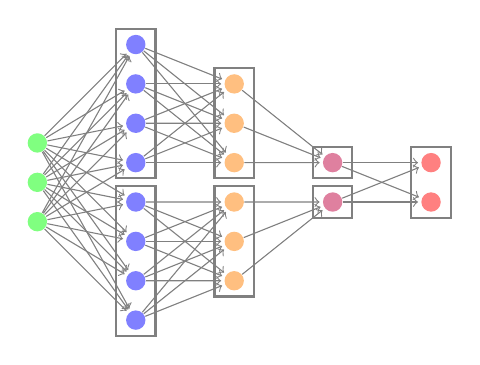
\begin{tikzpicture}[shorten >=1pt,->,draw=black!50, node distance=\layersep]
    \tikzstyle{every pin edge}=[<-,shorten <=1pt]
    \tikzstyle{neuron}=[circle,fill=black!25,minimum size=7pt,inner sep=0pt]
    \tikzstyle{rect}= [rectangle, draw=black!50, thick, minimum width=0.5cm, minimum height=1.7cm]
    \tikzstyle{input neuron}=[neuron, fill=green!50];
    \tikzstyle{output neuron}=[neuron, fill=red!50];
    \tikzstyle{hidden neuron}=[neuron, fill=blue!50];
    \tikzstyle{hidden neuron2}=[neuron, fill=orange!50];
    \tikzstyle{hidden neuron3}=[neuron, fill=purple!50];
    \tikzstyle{annot} = [text width=4em, text centered]

    % Draw the input layer nodes
    \foreach \name / \y in {1,...,3}
    % This is the same as writing \foreach \name / \y in {1/1,2/2,3/3,4/4}
    \node[input neuron] (I-\name) at (0,-\y/2-0.25) {};

    % Draw the hidden layer nodes
    \foreach \name / \y in {1,...,8}
    \path[yshift=2cm]
    node[hidden neuron] (H-1-\name) at (\layersep,-\y/2-1) {};
    \node[rect, minimum height=1.9cm] (L1-1) at (\layersep,-0.25) {};
    \node[rect, minimum height=1.9cm] (L1-2) at (\layersep,-2.25) {};
    \foreach \name / \y in {1,...,6}
    \path[yshift=1.5cm]
    node[hidden neuron2] (H-2-\name) at (2*\layersep,-\y/2-1) {};
    \node[rect, minimum height=1.4cm] (L2-1) at (2*\layersep,-0.5) {};
    \node[rect, minimum height=1.4cm] (L2-2) at (2*\layersep,-2) {};
    \foreach \name / \y in {1,...,2}
    \path[yshift=0.5cm]
    node[hidden neuron3] (H-3-\name) at (3*\layersep,-\y/2-1) {};
    \node[rect, minimum height=0.4cm] (L3-1) at (3*\layersep,-1) {};
    \node[rect, minimum height=0.4cm] (L3-1) at (3*\layersep,-1.5) {};
    % Draw the output layer node
    \foreach \name / \y in {1,...,2}
    \path[yshift=0.5cm]
    node[output neuron] (O-\name) at (4*\layersep,-\y/2-1) {};
    \node[rect, minimum height=0.9cm] (L4) at (4*\layersep,-1.25) {};

    % Connect every node in the input layer with every node in the
    % hidden layer.
    \foreach \source in {1,...,3}
    \foreach \dest in {1,...,8}
    \path (I-\source) edge (H-1-\dest);

    \foreach \source in {1,...,4}
    \foreach \dest in {1,...,3}
    \path (H-1-\source) edge (H-2-\dest);
    \foreach \source in {5,...,8}
    \foreach \dest in {4,...,6}
    \path (H-1-\source) edge (H-2-\dest);

    % Connect every node in the hidden layer with the output layer
    \foreach \source in {1,...,2}
    \foreach \dest in {1,...,2}
    \path (H-3-\source) edge (O-\dest);

    \foreach \source in {1,...,3}
    \foreach \dest in {1,...,1}
    \path (H-2-\source) edge (H-3-\dest);
    \foreach \source in {4,...,6}
    \foreach \dest in {2,...,2}
    \path (H-2-\source) edge (H-3-\dest);

    % Annotate the layers
    %\node[annot,above of=H-1-1, node distance=0.5cm] (hl) {Layer 1};
    %\node[annot,left of=hl] {Input};
    %\node[annot,above of=H-2-1, node distance=1cm](hl2) {Layer 2};
    %\node[annot,right of=hl2](hl3) {Layer 3};
    %\node[annot,right of=hl3](hl4) {Layer 4};
\end{tikzpicture}
